\documentclass{sig-alt-release2}
\usepackage{url}
\usepackage{color}
\usepackage{graphics,graphicx}

\usepackage{epsfig}
\usepackage{epstopdf}

\usepackage{colortbl}
\usepackage{multirow}
\usepackage{booktabs}
\usepackage{ifthen}  

\begin{document}
\newcommand{\todo}[1]{\textcolor{red}{#1}}
\def\newblock{\hskip .11em plus .33em minus .07em}

\conferenceinfo{DIM3} {2010, Glasgow, UK} 
\CopyrightYear{2010}
\clubpenalty=10000
\widowpenalty = 10000

\title{{Report Name}}

\numberofauthors{1}
\author{
\alignauthor
Author Names\\
	   \affaddr{Team D}\\
      \affaddr{Dim3}\\
      \affaddr{Fiona Buyers, Christopher James, Ryan Wells}\\
             \email{\{1003648b, 1003019j, 1002253w \}@students.glasgow.ac.uk }
}
\maketitle

\begin{abstract}
A multi-player game designed to encourage a balance between personal gain and the well being of a group.

\end{abstract}

\section{Aim of Application}

\subsection{Application Purpose}

The application itself is a multi-player game designed to encourage users to work effectively as part of a group. When users register they will be randomly assigned to one of four factions. Whilst playing the user will aim to increase not only their individual score, but the score of their faction. To do this, the user will have to buy buildings to expand their `city' and increase their population. There will be several different kinds of buildings; farms, barracks, studios and labs; each earning the user points in a different category (food, military, art and science, respectively) and all these buildings will earn money as time progresses. Points earned by the user will be added to the total for the relevant faction and the four faction totals will be displayed, showing which faction is the strongest in each area. Crisis events will occur throughout the game which will cause buildings of a certain kind to become less or more effective, for example famine or war, so in order for the user to have a successful city and gain the maximum number of points, the city they have created should be as well balanced as possible. More accomplished users will be able to unlock different personas when they have enough money, giving the user different multipliers for each of the points categories, affecting the amount of points earned for the faction. The majority of personas will not only feature positive multipliers, but also some that are detrimental to point production. This will allow users to choose what their city will focus on in terms of the types of points they wish to earn, but will also encourage users to continue playing as regular expansions of cities will be required to enable a user to afford a change in persona. The default persona is the `civilian' persona, which provides no multipliers for points or money, users who have purchased a persona are able to return to `civilian' status for free whenever they choose.

\subsection{Assumptions}

What are the assumptions about the aims and objectives?
- not having more than one account
- not losing password
- have a basic understanding of how this kind of game works
-

\subsection{Design Goals and Objectives} 

Describe the design goals and objectives of the application.
-

\subsection{Constraints}

What are the constraints of the project?
-

\subsection{Functional Requirements}

Functionality List: i.e. what is the required and desired functionality?

\begin{itemize}

\item The user's individual score should be tracked.

\item The individual score should affect the appropriate team's overall score.

\item Upon registration, the user should be randomly assigned a faction.

\item The amount of money a user currently has should be tracked and the user should not be allowed to buy buildings or personas that cost more than they have, and when an item is bought the amount of money possessed should be altered appropriately.

\item Users should earn money and points from their current buildings at set time intervals.

\item Users should be able to purchase several different kinds of building and persona if they have enough money.

\item Users should be able to return to civilian status for free whenever they want.

\item The faction scores page should be accessible both from the login page to users who are no logged in, and from the main game screen.

\item The faction scores page should show the percentage of the total number of points each faction has.

\end{itemize}

\subsection{stuff to do} 

Reflective Questions: 
Is the scope of the application appropriate? 
Are the design goals realistic/achievable? 
How complex is the application? 
Is distribution across the web appropriate? 

\section{Client Interface}

\subsection{User Interface}

Draw a wireframe of the user interface 
this may require several wireframes depending on the complexity of the application and the interfaces {\bf *need diagrams*} 

Describe the user interface.
i.e. Label key input and output components: describe them. {\bf *need diagrams*} 

Is the user interface intuitive, appealing, usable, etc?

Provide a Walkthrough and explain the user interactions with application. 
i.e. use cases AAAAAAAAARGH {\bf *need diagrams*} \\

The user interface was primarily designed to provide a fluid and natural experience to the user. When considering the user experience, care was taken to ensure that the interface was attractive to users but still provided enough functionality on each layer such that users could fulfil all the relevant tasks they wished to without having to change page an excessive amount of times. \\

\begin{figure}[!htbp]
  \caption{\textit{Login Page}}
  \begin{center}
		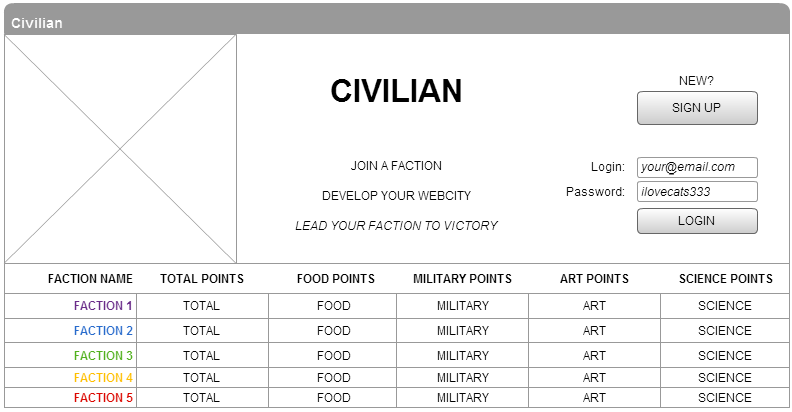
\includegraphics[scale=0.25]{img/w3.png}
  \end{center}
\end{figure}

\begin{figure}[!htbp]
  \caption{\textit{Game Page}}
  \begin{center}
		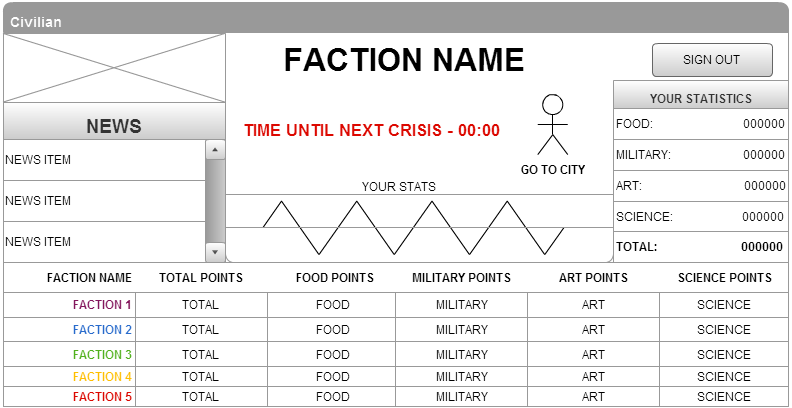
\includegraphics[scale=0.25]{img/w4.png}
  \end{center}
\end{figure}

The interface mostly followed the wireframes originally drawn up, but changes were made following feedback from the presentation earlier in the Semester. The initial design of the application (shown in Figures 1 and 2) had two main pages, a login page, allowing users to login, register and view the current faction scores, and a game page, showing the current users statistics and the buildings the currently owned, along with the current faction scores. Before implementation, this was changed slightly so that the current faction scores are shown in a separate page and both the login and game screens were redesigned slightly, these are shown in figures 204834 - 7174751.\\

\begin{figure}[!htbp]
  \caption{\textit{Total Faction Points Page}}
  \begin{center}
		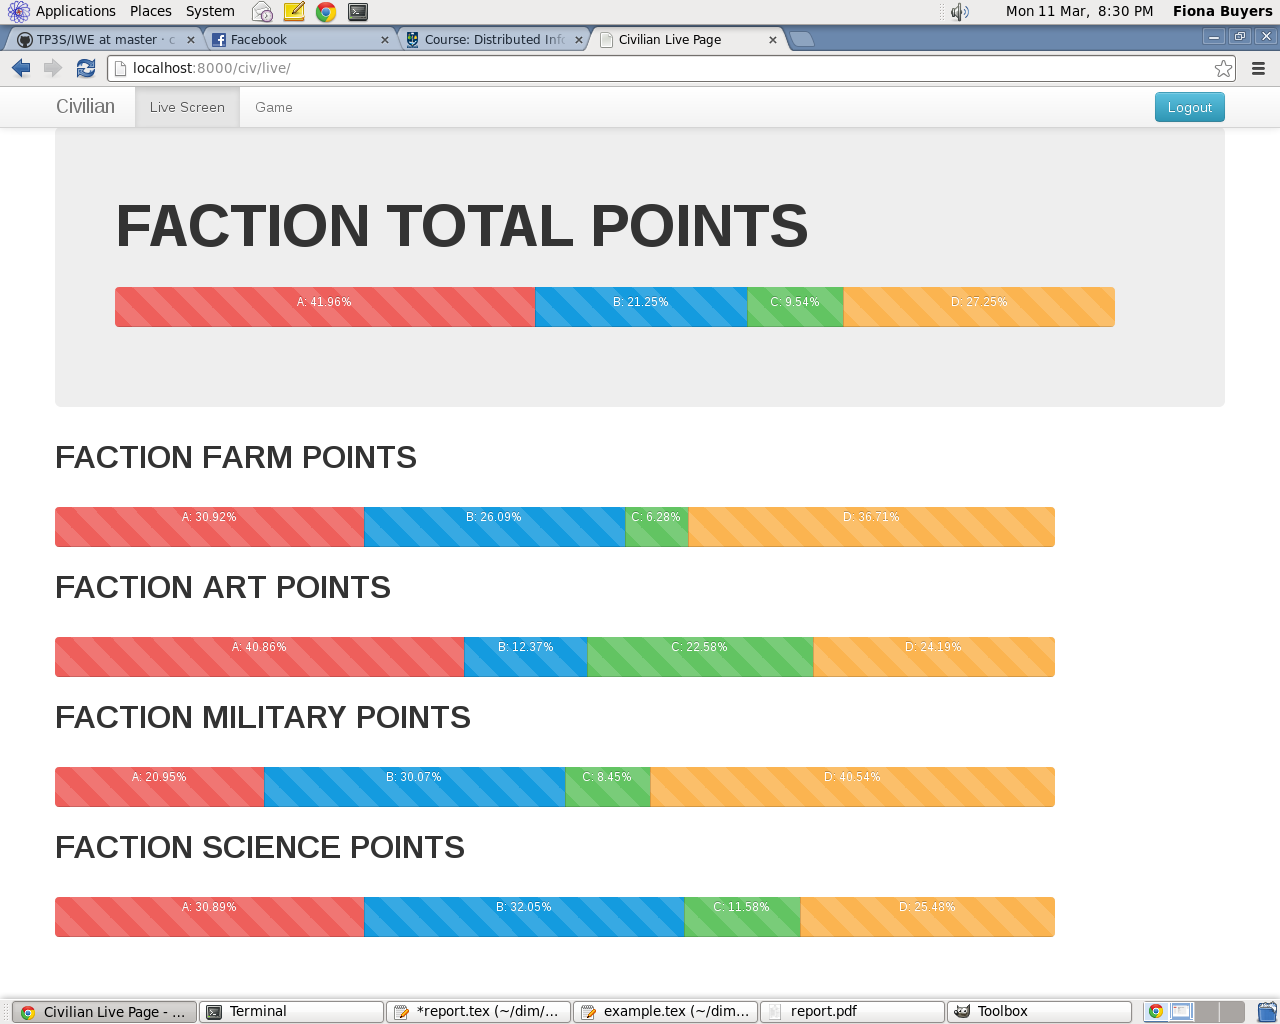
\includegraphics[scale=0.15]{img/faction.png}
  \end{center}
\end{figure}

\begin{figure}[!htbp]
  \caption{\textit{Game Page}}
  \begin{center}
		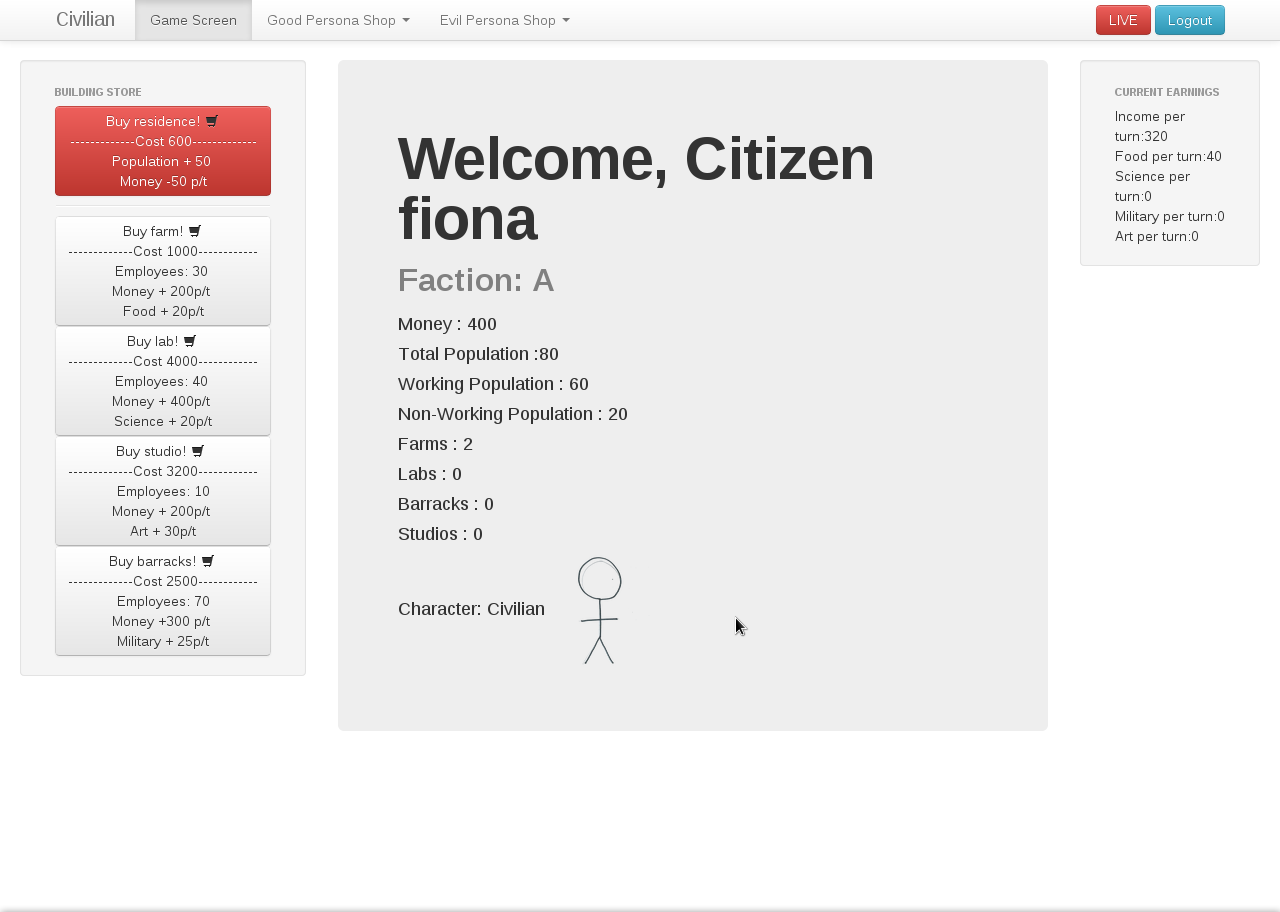
\includegraphics[scale=0.15]{img/gamescreen.png}
  \end{center}
\end{figure}

\begin{figure}[!htbp]
  \caption{\textit{Index Page}}
  \begin{center}
		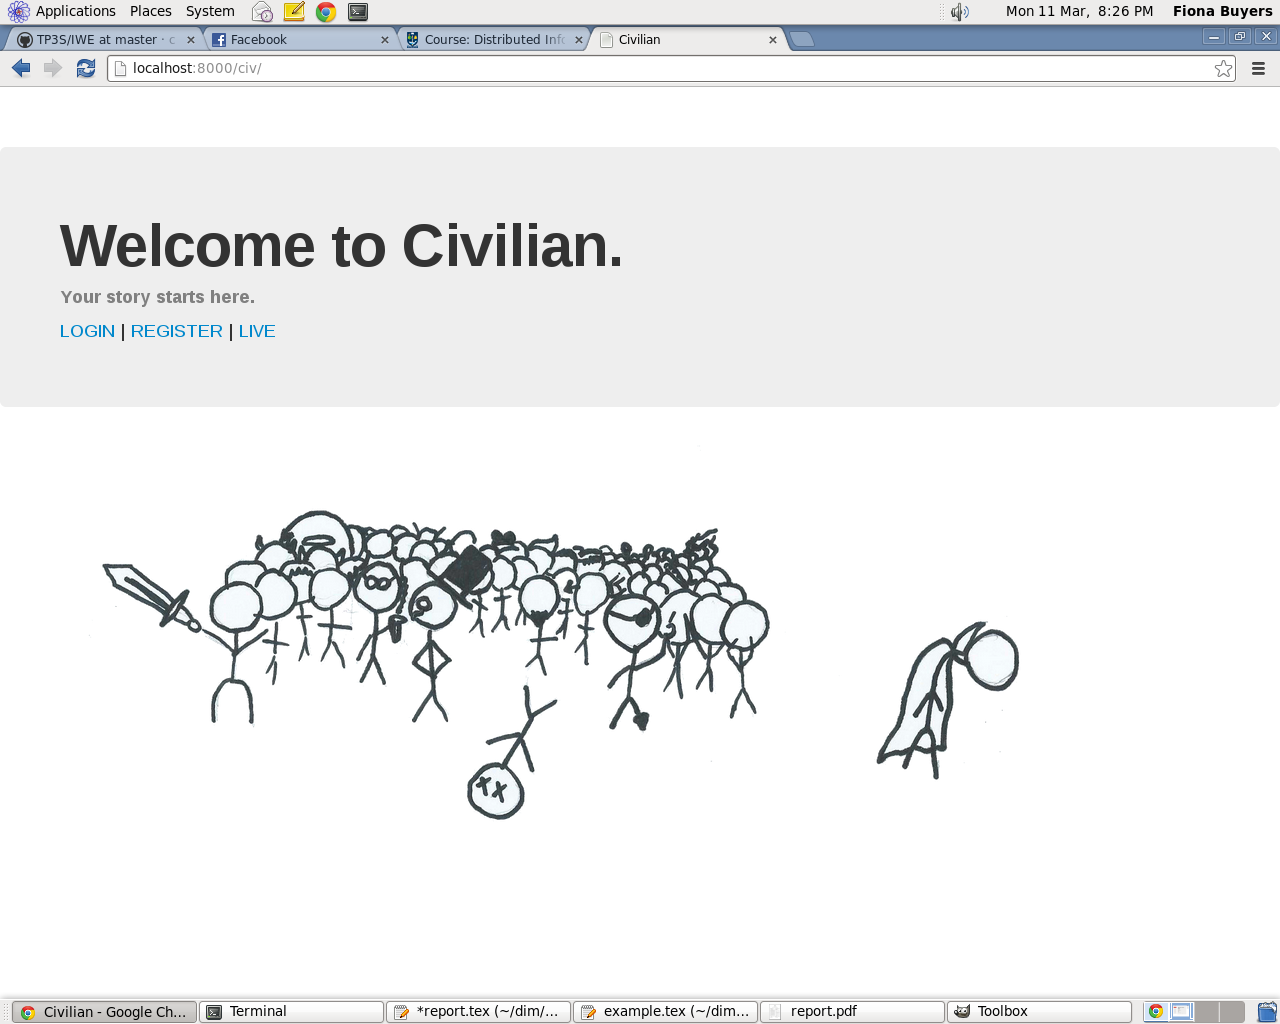
\includegraphics[scale=0.15]{img/index2.png}
  \end{center}
\end{figure}

\begin{figure}[!htbp]
  \caption{\textit{Register Page}}
  \begin{center}
		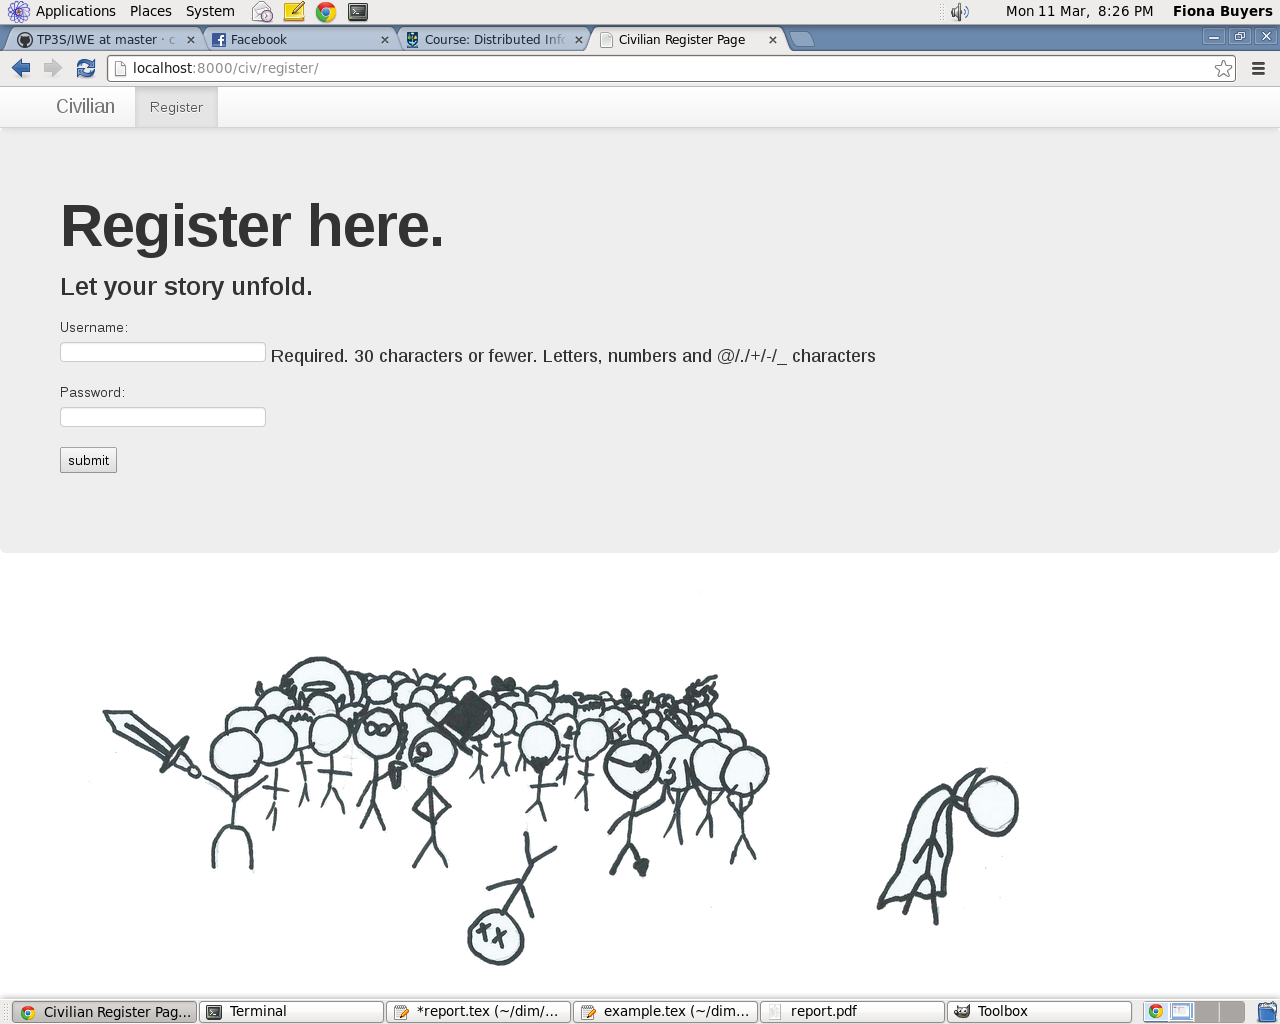
\includegraphics[scale=0.15]{img/register.png}
  \end{center}
\end{figure}

\begin{figure}[!htbp]
  \caption{\textit{Login Page}}
  \begin{center}
		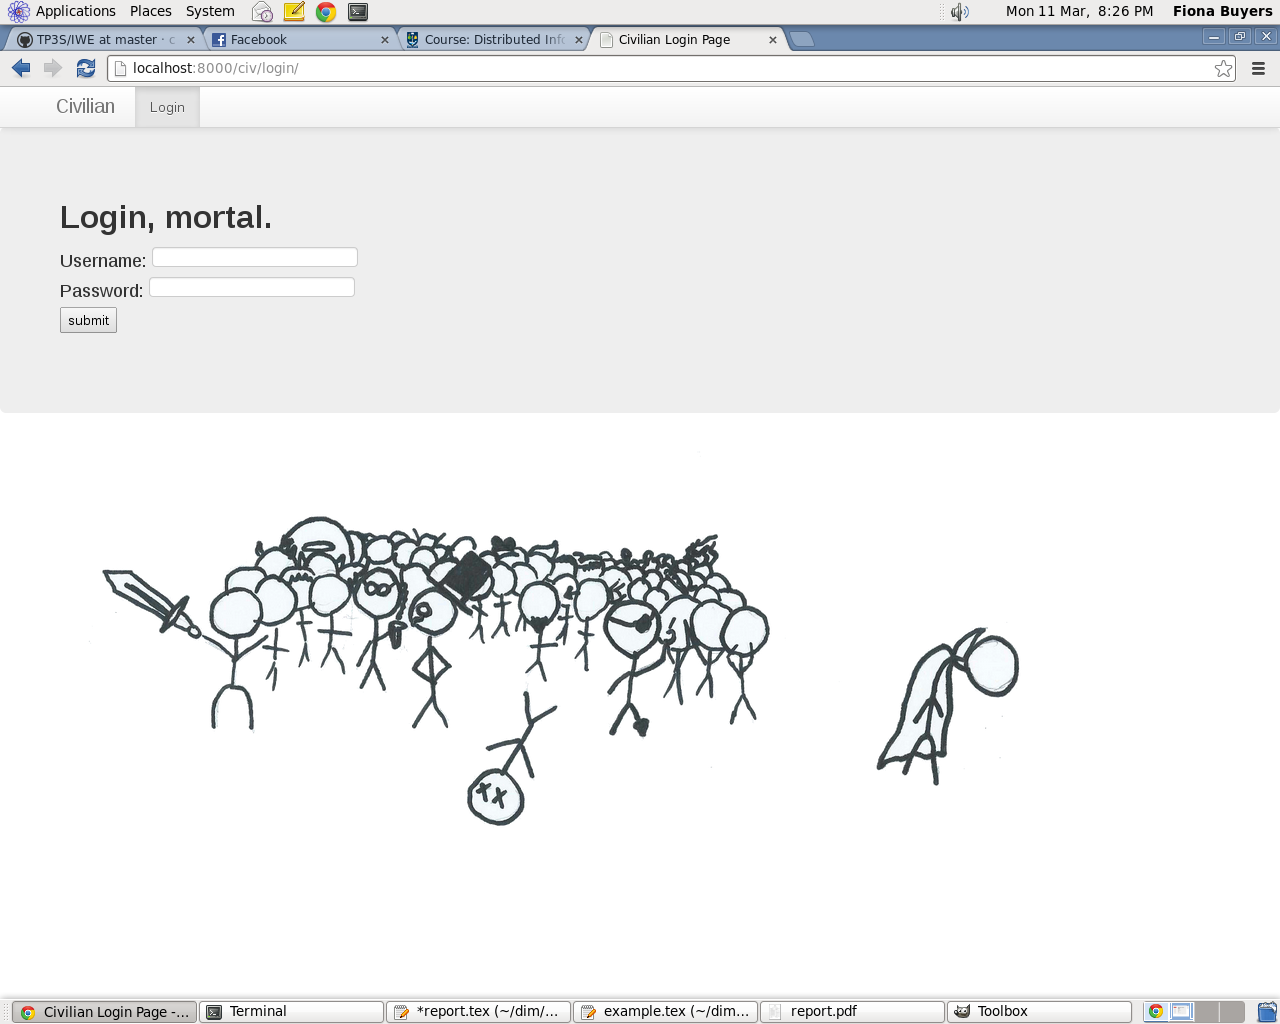
\includegraphics[scale=0.15]{img/login.png}
  \end{center}
\end{figure}

There final design has three main screens: the index page, the game page and the faction scores page. The index  page, provides options to login, register or view the current faction scores. The faction scores page shows the faction that currently has the most money, and also the greatest number of points for each of the categories. This page is accessible from within the game and without logging in, allowing unregistered players the ability to monitor the factions' scores. The main game page shows the current number of buildings each user has, displays their current points and how much money they will earn each turn. Users will also be able to purchase buildings for their city, and personas from this page. 

\subsection{Dynamic Components}

Describe the interactions associated with the dynamic components on the user interface.
What calls are required to dynamically update the data on the client side?
How does the user interface help the user achieve their goal, or complete their task? 

Due to the nature of the application, frequent updating of the database is required. The majority of the updating done to the client side uses Ajax GET requests, some at a timed interval, some whenever a user performs a specific event, such as purchasing a building.

\subsection{stuff to do} 

What technologies are used on the client side? 
What are the reasons for your choices? i.e. what is the advantages and disadvantages of using this technology? 
What other options are there? 

\section{Application Architecture}

\subsection{N-Teir Architecture Diagram}

N-Teir Architecture Diagram - chris has this {\bf *need diagrams*} 
i.e. data flow diagram between the interface/client, middle ware, and backend services/data repos

Describe the data model i.e. what data needs to be stored or persisted by the application? i dont even know what this is

\subsection{Entity-Relationship Diagram}

What are the relationships within the data model.
i.e. use ER diagram and explain. {\bf *need diagrams*} 

\subsection{Backend Services}

Describe the backend services used (if any).

\subsection{stuff to do} 

Reflective Questions: 
How have you ensured that there is a separation of concerns? 
What other technology could have been used instead of django? 
What are the advantages of using a Web Application Framework over other technology? 
And, what are the disadvantages?

\section{Message Parsing}

\subsection{Sequence Diagrams}

On the architecture diagram, identify and label the main messages that will be parsed through the application.
or alternatively (and preferably) include sequence diagrams to denote the sequence of communications parse between clients and servers. {\bf *need diagrams*} 

Describe the messages that are parsed back and forth through the application.

\subsection{Message Payload}

For the main transactions - describe the payload of the messages 
i.e. What are the contents of the messages? i.e. include sample XML, XHTML, JSON, etc of one or two messages.

\subsection{Message Format}

What is the format of the messages? 
Why this format? 
What other formats could be used, what are the advantages and disadvantages of these other formats?

\section{Implementation Notes}

\subsection{Views}

Views - What are the main views that you have implemented and what do they do?

\subsection{URL Mapping Schema}

URL Mapping Schema - what is your URL mapping and schema?

\subsection{External Services}

External Services  - what external services does your application include and what handlers did you include?

\subsection{Functionality Checklist}

Functionality Checklist (which functionality is completed) - everything except crises

\subsection{Known Issues}

Known Issues (what kind of works, what kind of errors to do you get)

\subsection{Technologies Used}

What technologies have been used and are required for the application. Include a list or table of all the technologies, standards, and protocols that will be required.

\section{Reflective Summary}

For the Implementation Report Only:
What have you learnt through the process of development? 
How did the application of frameworks help or hinder your progress?
What problems did you encounter? - timing?
What were your major achievements?


\section{Summary and Future Work}

Summary of application and its current state.

Include a list or table of all the technologies, standards, and protocols that will be required.

What are the limitations?

Plans for future development - crisis events, more personas and buildings.

The application 

\section{Acknowledgements}
Our thanks to Lief and Euan for their comments, suggestions and interest they showed in the project throughout the duration of the course. And our thanks to the peer reviewers for their feedback.
Thanks also go to Tom Whitely for his evaluation of the interface and the suggestions he made.

\bibliographystyle{abbrv}
\bibliography{sig-proc}

\end{document}
